% Readaptado de Semana 08 Clase 01 (2025-A), con ejemplos geometricos de 2026B.
\documentclass[compacto,10pt]{pubciencias-notas}
\usepackage{comandosEPN}
\usepackage{tikz}
\usetikzlibrary{babel}
\autor{Departamento de Formación Básica}
\materia{Álgebra Lineal}
\nota{Semana 07 Clase 02}
\fecha{Semestre 2026-B}
\logouno[1.1cm]{Logo_EPN.eps}
\logodos[1.7cm]{Logo_DFB.eps}
\definecolor{colordef}{cmyk}{0.81,0.62,0.00,0.22}
\raggedbottom

\begin{document}
\encabezado
\vspace*{-8mm}
\setcounter{section}{3}
\section{Espacios vectoriales}
\subsection{Combinación lineal}

En la clase anterior describimos rectas y planos mediante ecuaciones y
parámetros. Ahora construiremos vectores sumando múltiplos de otros
vectores. En toda la clase los escalares son reales.

\begin{defi}[Combinación lineal]\label{sem07cl02:combinacion}
    Sean $v_1,\ldots,v_k$ vectores de un espacio vectorial real $V$.
    Un vector $w\in V$ es una \textbf{combinación lineal} de ellos si
    existen escalares $\alpha_1,\ldots,\alpha_k\in\R$ tales que
    \[
        w=\alpha_1v_1+\cdots+\alpha_kv_k.
    \]
    Los $\alpha_i$ son los coeficientes de la combinación. Pueden ser
    positivos, negativos o cero.
\end{defi}

\begin{ejem}
    Sean $u=(1,0)$, $v=(1,1)$ y $w=(3,2)$ vectores de $\R^2$.
    Probemos que $w$ es una combinación lineal de $u$ y $v$.
    Para ello, buscamos escalares $a,b\in\R$ tales que
    \[
        w=au+bv=a(1,0)+b(1,1)=(a+b,b).
    \]
    Al igualar las componentes con las de $w=(3,2)$, obtenemos el sistema
    \[
        \left\{\begin{aligned}a+b&=3,\\b&=2.\end{aligned}\right.
    \]
    De la segunda ecuación, $b=2$; al sustituir en la primera, $a=1$.
    Por tanto, $w=u+2v$, lo que demuestra que $w$ es una combinación
    lineal de $u$ y $v$ con coeficientes 1 y 2, respectivamente.
\end{ejem}
\begin{center}
    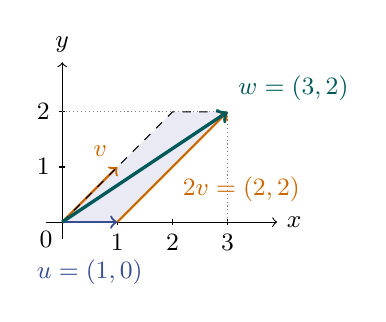
\begin{tikzpicture}[scale=0.7,every node/.style={font=\small}]
        \draw[->] (-0.3,0)--(3.9,0) node[right] {$x$};
        \draw[->] (0,-0.3)--(0,2.9) node[above] {$y$};
        \foreach \x in {1,2,3}
            \draw (\x,0.05)--(\x,-0.05) node[below] {$\x$};
        \foreach \y in {1,2}
            \draw (0.05,\y)--(-0.05,\y) node[left] {$\y$};
        \fill[colordef!8] (0,0)--(1,0)--(3,2)--(2,2)--cycle;
        \draw[densely dotted,gray] (3,0)--(3,2)--(0,2);
        \draw[->,thick,colordef] (0,0)--(1,0)
            node[midway,below=10pt] {$u=(1,0)$};
        \draw[->,thick,orange!80!black] (0,0)--(1,1)
            node[above left] {$v$};
        \draw[->,thick,orange!80!black] (1,0)--(3,2)
            node[midway,below right] {$2v=(2,2)$};
        \draw[dashed] (0,0)--(2,2)--(3,2);
        \draw[->,very thick,teal!70!black] (0,0)--(3,2)
            node[above right] {$w=(3,2)$};
        \node[below left] at (0,0) {$0$};
    \end{tikzpicture}
\end{center}

\subsection{Cápsula lineal e interpretación geométrica}
\begin{defi}[Cápsula lineal]\label{sem07cl02:capsula}
    Sea $S=\{v_1,\ldots,v_k\}\subseteq V$. La \textbf{cápsula lineal}
    o \textbf{subespacio generado por $S$}, denotado $\spn(S)$, es el
    conjunto de todas las combinaciones lineales de sus vectores:
    \[
        \spn(S)=\left\{v\in V:
            \begin{array}{l}
                \text{existen }\alpha_1,\ldots,\alpha_k\in\R
                \text{ tales que}\\
                v=\alpha_1v_1+\cdots+\alpha_kv_k
            \end{array}\right\}.
    \]
    Una combinación es un vector; la cápsula es un conjunto de vectores.
\end{defi}

\begin{ejem}[Calcular la cápsula mediante un sistema]\label{sem07cl02:recta}
    Sean $u=(2,3)$ y $v=(4,6)$. Determine la cápsula lineal
    $\spn\{u,v\}$ e interprete geométricamente el resultado.

    \textbf{Solución.} Sea $S=\{u,v\}$. Por la definición de cápsula,
    \[
        \spn(S)=\left\{(x,y)\in\R^2:
            \begin{array}{l}
                \text{existen }a,b\in\R\text{ tales que}\\
                (x,y)=au+bv
            \end{array}\right\}.
    \]
    Para determinar qué vectores $(x,y)$ cumplen esta condición,
    sustituimos $u=(2,3)$ y $v=(4,6)$ en la combinación lineal:
    \[
        (x,y)=a(2,3)+b(4,6)=(2a+4b,3a+6b).
    \]
    Igualar componentes da el sistema en las incógnitas $a,b$:
    \[
        \left\{\begin{aligned}2a+4b&=x,\\3a+6b&=y.\end{aligned}\right.
    \]
    Reducimos su matriz ampliada mediante $2F_2-3F_1\rightarrow F_2$:
    \[
        \left(\begin{array}{cc|c}2&4&x\\3&6&y\end{array}\right)
        \sim
        \left(\begin{array}{cc|c}2&4&x\\0&0&2y-3x\end{array}\right).
    \]
    La matriz de coeficientes tiene rango 1. Si $2y-3x\ne0$, la matriz
    ampliada tiene rango 2 y el sistema no tiene solución. Si $2y-3x=0$,
    ambos rangos son 1 y el sistema sí tiene solución. Por tanto,
    \[
        \boxed{\spn\{u,v\}=\{(x,y)\in\R^2:3x-2y=0\}.}
    \]
    Las coordenadas $x,y$ describen el vector que queremos construir;
    las incógnitas del sistema son sus coeficientes $a,b$.
\end{ejem}

\begin{defi}[Conjunto generador]\label{sem07cl02:generado}
    Sea $S=\{v_1,\ldots,v_k\}\subseteq V$.
    Decimos que $S$ es un \textbf{conjunto generador de $V$} si cada vector
    de $V$ es una combinación lineal de los elementos de $S$.
\end{defi}

\begin{teo}
    La cápsula $\spn(S)$ es el menor subespacio de $V$ que contiene a $S$:
    está contenida en cualquier subespacio de $V$ que contenga a todos
    los vectores de $S$. En particular, $S$ genera $V$ si y solo si
    $\spn(S)=V$.
\end{teo}
\begin{ejem}[Generar todo el plano]\label{sem07cl02:generarR2}
    Sean $u=(1,0)$ y $v=(1,1)$, como en el ejemplo anterior. Para determinar
    si generan $\R^2$, buscamos coeficientes para un vector arbitrario
    $(x,y)$:
    \[
        a(1,0)+b(1,1)=(x,y)
        \quad\Longleftrightarrow\quad
        \left\{\begin{aligned}a+b&=x,\\b&=y.\end{aligned}\right.
    \]
    Para todo $x,y\in\R$ hay solución: $a=x-y$ y $b=y$. Así,
    $(x,y)=(x-y)u+yv$ y
    $\spn\{u,v\}=\R^2$.
    A diferencia del ejemplo \ref{sem07cl02:recta}, no hay una restricción
    sobre las coordenadas del vector objetivo: se alcanza todo el plano.
\end{ejem}

\begin{ejem}[Un plano en $\R^3$]\label{sem07cl02:plano}
    Sean $a=(1,0,1)$ y $b=(0,1,1)$. Pruebe que
    $\spn\{a,b\}=P$, donde
    \[
        P=\{(x,y,z)\in\R^3:x+y-z=0\}.
    \]

    \textbf{Solución.} Tomemos $(x,y,z)\in P$ y busquemos escalares
    $s,t\in\R$ que permitan escribirlo como combinación de $a,b$:
    \[
        s(1,0,1)+t(0,1,1)=(x,y,z).
    \]
    Al efectuar las operaciones e igualar componentes, obtenemos
    \[
        (s,t,s+t)=(x,y,z)
        \quad\Longleftrightarrow\quad
        \left\{\begin{aligned}s&=x,\\t&=y,\\s+t&=z.\end{aligned}\right.
    \]
    Las dos primeras ecuaciones dan $s=x$ y $t=y$. La tercera también
    se cumple, pues $x+y=z$ para todo vector de $P$. Por tanto,
    $(x,y,z)=xa+yb$ y todo vector del plano pertenece a la cápsula.

    Además, cualquier combinación $sa+tb=(s,t,s+t)$ satisface la
    ecuación del plano, ya que $s+t-(s+t)=0$. Concluimos que
    \[
        \boxed{\spn\{a,b\}=P.}
    \]
    El vector $(2,-1,1)=2a-b$ pertenece al plano, pero $(0,0,1)$ no:
    no satisface su ecuación.
\end{ejem}
\begin{center}
    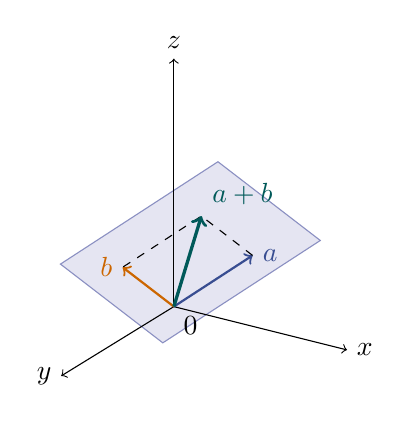
\begin{tikzpicture}[x={(1cm,-0.25cm)},y={(-0.65cm,-0.4cm)},z={(0cm,0.9cm)}]
        \filldraw[fill=colordef!10,draw=colordef!50]
            (-0.4,-0.4,-0.8)--(1.6,-0.4,1.2)--(1.6,1.6,3.2)--(-0.4,1.6,1.2)--cycle;
        \draw[->] (0,0,0)--(2.2,0,0) node[right] {$x$};
        \draw[->] (0,0,0)--(0,2.2,0) node[left] {$y$};
        \draw[->] (0,0,0)--(0,0,3.5) node[above] {$z$};
        \draw[->,thick,colordef] (0,0,0)--(1,0,1) node[right] {$a$};
        \draw[->,thick,orange!80!black] (0,0,0)--(0,1,1) node[left] {$b$};
        \draw[dashed] (1,0,1)--(1,1,2)--(0,1,1);
        \draw[->,very thick,teal!70!black] (0,0,0)--(1,1,2)
            node[above right] {$a+b$};
        \node[below right] at (0,0,0) {$0$};
    \end{tikzpicture}

    Al variar los dos coeficientes se recorre todo el plano, no solo el paralelogramo.
\end{center}

\subsection{Dependencia e independencia lineal}
\begin{defi}[Dependencia e independencia lineal]\label{sem07cl02:independencia}
    Un conjunto $S=\{v_1,\ldots,v_k\}$ de vectores de $V$ es
    \textbf{linealmente independiente (LI)} si la igualdad
    \[
        \alpha_1v_1+\cdots+\alpha_kv_k=0_V
    \]
    solo se cumple cuando $\alpha_1=\cdots=\alpha_k=0$.
    Es \textbf{linealmente dependiente (LD)} si existen coeficientes
    \textbf{no todos nulos} que producen esa igualdad.
\end{defi}

\begin{ejem}[Una relación de dependencia]
    Para $u=(2,3)$ y $v=(4,6)$ del ejemplo \ref{sem07cl02:recta},
    estudiamos si existen escalares $\alpha,\beta\in\R$, no ambos cero,
    tales que $\alpha u+\beta v=(0,0)$. Sustituimos los vectores y
    efectuamos las operaciones por componentes:
    \[
        \begin{aligned}
            \alpha(2,3)+\beta(4,6)&=(0,0),\\
            (2\alpha,3\alpha)+(4\beta,6\beta)&=(0,0),\\
            (2\alpha+4\beta,3\alpha+6\beta)&=(0,0).
        \end{aligned}
    \]
    Dos vectores son iguales si sus componentes correspondientes son
    iguales. Al igualar la primera componente a cero y luego la segunda,
    obtenemos el sistema homogéneo en las incógnitas $\alpha,\beta$:
    \[
        \left\{\begin{aligned}2\alpha+4\beta&=0,\\3\alpha+6\beta&=0.\end{aligned}\right.
    \]
    El sistema tiene rango 1 y dos incógnitas: $\alpha=-2\beta$.
    Tiene soluciones no triviales; por ejemplo, $\alpha=2$, $\beta=-1$.
    Así, $2u-v=0$ demuestra que el conjunto $\{u,v\}$ es LD.
\end{ejem}

\begin{prop}[Quitar un vector redundante]
    Si un vector de un conjunto es combinación lineal de los demás,
    quitarlo no cambia la cápsula. A ese vector lo llamamos redundante.
\end{prop}

Con $a,b$ del ejemplo \ref{sem07cl02:plano}, el vector $c=a+b$ es redundante:
$ra+sb+tc=(r+t)a+(s+t)b$. Por tanto,
$\spn\{a,b,c\}=\spn\{a,b\}$ y el conjunto $\{a,b,c\}$ es LD, pues
$a+b-c=0$ es una relación con coeficientes no todos nulos.

\begin{ejem}[Comprobar independencia]
    Para $u=(1,0)$ y $v=(1,1)$,
    \[
        \alpha u+\beta v=0
        \quad\Longleftrightarrow\quad
        (\alpha+\beta,\beta)=(0,0).
    \]
    La segunda componente da $\beta=0$ y la primera, $\alpha=0$.
    El conjunto $\{u,v\}$ es LI.
\end{ejem}

\begin{obs}[Relación con el rango]
    En $\R^n$, para $S=\{v_1,\ldots,v_k\}$ y
    $A=[\,v_1\ \cdots\ v_k\,]$, el conjunto $S$ es LI si
    y solo si $Ac=0$ tiene únicamente la solución trivial; equivalentemente,
    si $\rang(A)=k$. Si $\rang(A)<k$, el conjunto $S$ es LD.
    Solo para matrices cuadradas se puede usar directamente $\det(A)\ne0$.
\end{obs}
\begin{obs}[Consecuencias y precauciones]
    \leavevmode\par
    \begin{itemize}[leftmargin=*,labelsep=0.5em]
        \item Un conjunto que contiene al vector cero es LD: asígnele
              coeficiente 1 y a los demás coeficiente 0.
        \item Dos vectores no nulos son LD si uno es múltiplo del otro.
        \item Tres vectores pueden ser LD sin que ningún par sea paralelo:
              ocurre con $a,b,a+b$. Hay que estudiar el conjunto completo.
        \item Un conjunto LD tiene algún vector redundante: en una relación
              no trivial, despeje un vector cuyo coeficiente sea distinto de cero.
        \item Generar y ser LI son preguntas distintas: $a,b$ son LI en
              $\R^3$, pero generan un plano, no todo $\R^3$.
    \end{itemize}
\end{obs}

\subsection{Ejemplos con matrices y polinomios}

\begin{ejem}[Generar matrices diagonales]
    En $\Mat[\R]{2}{2}$, sean
    \[
        A=\begin{pmatrix}1&0\\0&1\end{pmatrix},\qquad
        B=\begin{pmatrix}1&0\\0&-1\end{pmatrix}.
    \]
    Determine su cápsula y decida si el conjunto $\{A,B\}$ es LI.

    \textbf{Solución.} Para $\alpha,\beta\in\R$,
    \[
        \alpha A+\beta B=
        \begin{pmatrix}\alpha+\beta&0\\0&\alpha-\beta\end{pmatrix}.
    \]
    Todas las combinaciones son diagonales. Tomemos una matriz diagonal
    genérica
    \[
        M=\begin{pmatrix}x&0\\0&y\end{pmatrix},\qquad x,y\in\R.
    \]
    Para escribir $M$ como combinación de $A$ y $B$, planteamos
    \[
        \alpha A+\beta B=M
        \quad\Longleftrightarrow\quad
        \begin{pmatrix}\alpha+\beta&0\\0&\alpha-\beta\end{pmatrix}
        =\begin{pmatrix}x&0\\0&y\end{pmatrix}.
    \]
    Al igualar las entradas correspondientes, obtenemos el sistema
    \[
        \left\{\begin{aligned}\alpha+\beta&=x,\\\alpha-\beta&=y.\end{aligned}\right.
        \quad\Longrightarrow\quad
        \alpha=\frac{x+y}{2},\quad\beta=\frac{x-y}{2}.
    \]
    Hay solución para todos $x,y\in\R$. En consecuencia,
    \[
        \spn\{A,B\}=
        \left\{\begin{pmatrix}x&0\\0&y\end{pmatrix}:x,y\in\R\right\}.
    \]
    Para la combinación nula, $x=y=0$, las únicas soluciones son
    $\alpha=\beta=0$. Por tanto, $A,B$ son LI, pero no generan todas
    las matrices de $\Mat[\R]{2}{2}$: ninguna combinación tiene entradas
    no nulas fuera de la diagonal.
\end{ejem}

\begin{ejem}[Polinomios: generar y eliminar redundancias]
    En $\Pol_2$, considere $S=\{1,t,t^2,1-2t\}$.
    Determine su cápsula y decida si $S$ es LI o LD.

    \textbf{Solución.} Todo polinomio $p(t)=a_0+a_1t+a_2t^2$ es una
    combinación de los tres primeros elementos:
    \[
        p(t)=a_0\cdot1+a_1t+a_2t^2+0(1-2t).
    \]
    Por tanto, $\spn(S)=\Pol_2$. Sin embargo,
    \[
        1-2t=1\cdot1-2\cdot t+0\cdot t^2,
    \]
    así que el cuarto polinomio es redundante. La igualdad
    $1\cdot1-2\cdot t+0\cdot t^2-1(1-2t)=0_{\Pol_2}$ demuestra que
    $S$ es LD: los coeficientes $(1,-2,0,-1)$ no son todos cero.

    Al quitar $1-2t$, queda el conjunto generador $\{1,t,t^2\}$.
    Para comprobar su independencia, planteamos
    \[
        \alpha\cdot1+\beta t+\gamma t^2=0_{\Pol_2}.
    \]
    Igualar los coeficientes de cada potencia da
    $\alpha=\beta=\gamma=0$; por tanto, este conjunto es LI.
    El cero de la igualdad es el polinomio idénticamente nulo,
    no el valor del polinomio en un solo punto.
\end{ejem}
\section{Ejercicios}

\begin{ejer}[Combinación y cápsula en el espacio]
    Sean $v_1=(3,0,-2)$ y $v_2=(2,-1,-5)$.
    \begin{enumerate}
        \item Determine para qué valor de $k$ el vector $(1,-2,k)$ es
              combinación lineal de $v_1,v_2$ y encuentre sus coeficientes.
        \item Calcule $\spn\{v_1,v_2\}$ planteando el sistema para un
              vector genérico $(x,y,z)$. Obtenga una ecuación del plano
              generado a partir de la condición de compatibilidad.
    \end{enumerate}
\end{ejer}

\begin{ejer}[Generación y dependencia en el plano]
    \begin{enumerate}
        \item Compruebe que $(1,3)$ y $(-2,4)$ son LI resolviendo la
              combinación nula. Determine si generan $\R^2$ planteando
              el sistema para un vector arbitrario $(x,y)$.
        \item Añada el vector $(-1,7)$ al conjunto anterior. Exhiba una
              relación de dependencia y explique por qué añadirlo no
              cambia el espacio generado.
    \end{enumerate}
\end{ejer}

\begin{ejer}[Cápsula de un conjunto de matrices]
    En $\Mat[\R]{2}{2}$, sean
    \[
        A=\begin{pmatrix}1&1\\0&0\end{pmatrix},\quad
        B=\begin{pmatrix}0&0\\0&1\end{pmatrix},\quad
        C=\begin{pmatrix}1&1\\0&1\end{pmatrix}.
    \]
    \begin{enumerate}
        \item Describa todas las matrices de $\spn\{A,B,C\}$ igualando
              entradas en una combinación lineal genérica.
        \item Decida si el conjunto es LI o LD. Identifique una matriz
              redundante y compruebe si las dos restantes son LI.
    \end{enumerate}
\end{ejer}

\begin{ejer}[Generar un espacio de polinomios]
    En $\Pol_2$, considere $S=\{1+t,1-t,t^2\}$.
    \begin{enumerate}
        \item Para $p(t)=a_0+a_1t+a_2t^2$, plantee
              $p(t)=\alpha(1+t)+\beta(1-t)+\gamma t^2$ e iguale
              coeficientes. Determine si $S$ genera $\Pol_2$.
        \item Estudie la combinación nula para decidir si $S$ es LI.
              Si se añade el polinomio 2, ¿cambian la cápsula y la
              independencia? Justifique con una relación explícita.
    \end{enumerate}
\end{ejer}

\end{document}
